%\documentclass[10pt,journal,compsoc]{IEEEtran}
\documentclass[conference]{IEEEtran}
\IEEEoverridecommandlockouts
% The preceding line is only needed to identify funding in the first footnote. If that is unneeded, please comment it out.
\usepackage{cite}
\usepackage{amsmath,amssymb,amsfonts}
\usepackage{graphicx}
\usepackage{textcomp}
\usepackage{xcolor}
\def\BibTeX{{\rm B\kern-.05em{\sc i\kern-.025em b}\kern-.08em
		T\kern-.1667em\lower.7ex\hbox{E}\kern-.125emX}}
\usepackage{float}

% *** SPECIALIZED LIST PACKAGES ***
%
\usepackage{algorithmic}

% *** ALIGNMENT PACKAGES ***
%
\usepackage{array}

% *** FLOWCHART AND GRAPHS PACKAGES ***
%
\usepackage{tikz}
\usetikzlibrary{snakes,arrows,shapes, shapes.geometric, calc, automata,positioning}
\tikzstyle{startstop} = [rectangle, rounded corners, minimum width=3cm, minimum height=1cm,text centered, trapezium stretches=true, draw=black, 
%fill=red!30
]
\tikzstyle{io} = [trapezium, trapezium left angle=70, trapezium right angle=110, minimum width=3cm, trapezium stretches=true, minimum height=1cm, text centered, draw=black, 
%fill=blue!30
]
\tikzstyle{process} = [rectangle, minimum width=3cm, minimum height=1cm, text centered, draw=black, trapezium stretches=true, 
%fill=orange!30
]
\tikzstyle{decision} = [diamond, minimum width=3cm, minimum height=1cm, text centered, draw=black, trapezium stretches=true, 
%fill=green!30
]
\tikzstyle{arrow} = [thick,->,>=stealth]

% *** TABLE RELATED CHANGES ***
%
\renewcommand\arraystretch{2}
\newcolumntype{L}{>{\arraybackslash}m{4cm}}
\newcolumntype{P}{>{\arraybackslash}m{2cm}}
\newcolumntype{C}{>{\arraybackslash}m{1.2cm}}

% IEEEtran contains the IEEEeqnarray family of commands that can be used to
% generate multiline equations as well as matrices, tables, etc., of high
% quality.

\usepackage{url}
\hyphenation{op-tical net-works semi-conduc-tor}

\newcommand\rtos{Real Time Operating System}
\newcommand\rtai{Real Time Application Interface}
\newcommand\rtlinux{RTLinux}
\newcommand\rtsS{Real time system }
\newcommand\rts{Real time system}

\makeatletter
\def\endthebibliography{%
    \def\@noitemerr{\@latex@warning{Empty `thebibliography' environment}}%
    \endlist
}
\makeatother
\graphicspath{{./graphics/}}


\begin{document}
%
% paper title
\title{Programming issues in Real Time Systems
%	{\footnotesize \textsuperscript{*}Note: Sub-titles are not captured in Xplore and should not be used}
%	\thanks{Identify applicable funding agency here. If none, delete this.}
}

\author{\IEEEauthorblockN{Gahan Saraiya}
	\IEEEauthorblockA{\textit{Institute of Technology} \\
		\textit{Nirma University}\\
		Ahmedabad, India \\
		18mcec10@nirmauni.ac.in}
	\and
	\IEEEauthorblockN{Rushi Trivedi}
	\IEEEauthorblockA{\textit{Institute of Technology} \\
		\textit{Nirma University}\\
		Ahmedabad, India \\
		18mcec08@nirmauni.ac.in}
}

% The paper headers
%\markboth{Consummating Research Projects using Agile Manifesto, November~2018}%
%{Shell \MakeLowercase{\textit{et al.}}: Consummating Research Projects using Agile Manifesto}

\maketitle
% make the title area
\IEEEdisplaynontitleabstractindextext
\IEEEpeerreviewmaketitle

\begin{abstract}
    The growth in industry has driven the requirement for Real Time systems over time for many applications. Majority applications are now days considered as Real Time Systems where some applications may result in catastrophic event. But Even though Response Time of every system are considered as base criteria for each and every systems from a small electronics chip or software to largely distributed applications or network containing cluster of hardware and software. Response Time is not just simple thing which can be achieved easily as the desire is to get minimum response time without loosing accuracy of the system. This is because of the various issues arises in design of real time systems due to programming, hardware architecture, operating system, network latency (if distributed) etc. This paper illustrates and focuses on programming issues arises for real time systems.
%    and solution to cope with the issues.
\end{abstract}

% Note that keywords are not normally used for peerreview papers.
\begin{IEEEkeywords}
	Real Time Systems, Programming issues
\end{IEEEkeywords}

%\IEEEraisesectionheading{\section{Introduction}\label{sec:introduction}}
\section{Introduction}\label{sec:introduction}
Designing \rts s is a challenging task as a growing requirements and expectations from systems. As Real time systems have to interact with real world entities most of the challenge comes from that. These interactions can get more and more complex. Typically a \rts might be interacting with thousands of such entities at the same time. For example, a telecom system routinely handles calls from thousands of people at the same moment. The system has to connect each call differently. Constraint like sequence of calls, amount of noise and quality of call availability of service etc.

For applications such as in air-traffic control system, satellite launching are considered as hard \rts because if deadlines which are not followed the system then it causes the catastrophic damage. For some other applications such as temperature reading response deadline is important but can be missed occasionally which is not desirable but not causing any catastrophic damage hence such applications are considered as soft \rts. Also some deadlines can start soft and later become hard. i.e., a $ 3 ms $ periodic reading on an aircraft pressure sensor is ideal but can be missed, however a $ 15 ms $ interval could cause catastrophe. A firm system such as weather forecast is one in which if the deadline is missed then no value for doing it later.

\begin{figure}[!htbp]
    \centering
    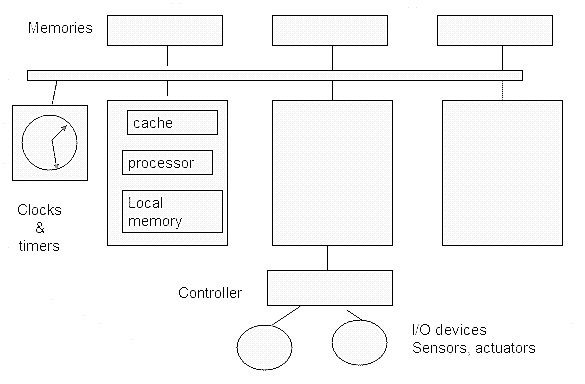
\includegraphics[width=0.5\textwidth]{genericsys.jpg}
    \caption{Generic Diagram of \rts\cite{realTimeIssues}}\label{fig:generic-rts}
\end{figure}

Components which are displayed in Fig. \ref{fig:generic-rts} are to be managed by program efficiently in such a way that maintains the accuracy of the system and achieve desire performance in terms of meeting deadline and response time.
\section{\rtsS Model}\label{section:rts-model}
A \rtsS model can be defined with below parameters:
\begin{itemize}
    \item Workload model (task graph) is about what behaviors system will be asked to perform
        \\ partially ordered set of tasks with timing information for each task where ordering represents dependency for the task
    \item Resource model (Capacity graph) is about tools and capabilities system applies
        \\ contains all of the passive resources that the system must use along with their acceptable patterns of use
    system resources are divided in to:
    \begin{itemize}
        \item Processors - active resources such as computers, database servers, etc.
        \item Resources - passive resources such as memory, semaphores, locks, other data.
    \end{itemize}
    \item Scheduling algorithm is about activity coordinated by system
        \\ considers the dependencies and interferences among the tasks
    \item Resource management algorithm
    \\ Activity coordinated by system
\end{itemize}

Each job in \rtsS can be defined as a unit work and set of such jobs together called as \textit{task set} achieves desired activity. Each and every job of task set runs on a processor and depends on some resources.
\rtsS job can be characterizes as:
\begin{itemize}
    \item temporal parameters
    \item functional parameters
    \item resource parameters
    \item interconnection parameters
\end{itemize}
Of course, the very important information for the real-time analysis are the timing prediction parameters. The execution time of jobs has many uncertainties due to following variable parameters:
\begin{itemize}
    \item execution - caches, pipelines
    \item internal - branches, loops
    \item external - preemption, interference
\end{itemize}
All of these issues lead to difficulties in making a priori decisions about how much time to allow, and promote the use of simulation models to help.

\section{Issues for Programming Environments}\label{section:issues-in-programming-environment}
For many years, job of real time system programmer is to write a program with an execution time which is lesser than the time constrained allowed. To predict the precise execution time of a program is very difficult hence it usually takes multiple rounds of trail and error method to build a reliable \rts. Also to port existing real-time software to a new configuration rather than building it from scratch takes the same level of effort which is not desirable since the requirements for real-time software are stronger than ever, because of ubiquity of computer systems in all application areas. And not only this but the next-gen real-time applications have more strict timing constraints.

To cope with such issues one needs to think of out-of-the box solution. Such an approach could be to make the system very flexible such that it can meet wide range of timing constraint under various system configurations. Thus the approach focuses on scalability for wide range of timing constraints rather than depending on precise execution time of computation.
In many hard real-time systems, the requirement for functional correctness is not as strict as the requirement for temporal correctness. For these applications, the flexible performance approach is thus preferred\cite{Lin1995}.

To design and develop the next generation \rtsS using approach described above, a programming language which has constructs for right away expressing timing constraints is required. The programmer defines the temporal constraints for the computation and also provides all possible set of codes to be executed. The runtime system along with the compiler and the scheduler must decide and/or generate the code for the execution so that the constraints are met.

Many language features are desirable for real-time systems programming. In fact, almost all features desirable in a "good" conventional (i.e., non-real-time) programming language can be considered as essential for real-time systems programming. For example, five requirements\label{rts-requirements} have been suggested for real-time software in \cite{Stoyenko1993}: \textit{predictability, reliability, tasking, modularity, and maintainability}. Other then predictability all remaining four are always highly desirable in every system. 

\subsection{Asynchronous Communication}
Remote procedure calls (RPC) are used in computer systems to simplify design of software. RPC allows a programmer to call procedures on a remote machine with the same semantics as local procedure calls. RPCs really ease the design and development of formal systems, but they are of very limited use in \rts s. The main reason is that mainly communication in the real world is asynchronous, i.e. only few message interactions can be classified into the query response prototype that works so well using RPCs.

Thus most \rts s support design based on state machine where multiple messages can be received in a single state. The contents of the received message determines the next state. State machines provide a much flexible mechanism to handle asynchronous message interactions. However the flexibility comes with its own complexities.

\subsection{Working with Distributed Architectures}
Most \rts s involve processing on many different nodes. The system itself distributes the load of processing among multiple processors. This raises several challenges for programmer:
\begin{itemize}
    \item Maintaining Consistency: to maintain consistency in data-structure is a challenge when multiple processors are involved in execution. Generally consistency is maintained by running data-structure audits.
    \item Initializing the System: Initializing the system with multiple processors is too much complicated than bringing up a single machine. 
    When a node finishes initialization, it will initiate software downloads for all the child nodes directly connected to it. This process goes on in an hierarchical fashion till the complete system is initialized.
    \item Inter-Processor Interfaces: One of the biggest headache in \rts s is defining and maintaining message interfaces. Defining of interfaces is complicated by ordering and padding rules for different byte in processors. Maintenance of interfaces is complicated by backward compatibility issues. For example if a cellular system changes the air interface protocol for a new breed of phones, it will still have to support interfaces with older phones.
    \item Load Distribution: When multiple processors and links are involved in message interactions distributing the load evenly can be a daunting task. If the system has evenly balanced load, the capacity of the system can be increased by adding more processors. Such systems are said to scale linearly with increasing processing power. But often designers find themselves in a position where a single processor or link becomes a bottle neck. This leads to costly redesign of the features to improve system scalability.
    \item Centralized Resource Allocation: Distributed systems may be running on multiple processors, but resources must be allocated from a shared pool. Shared pool allocation is typically managed by a single processor allocating resources from the shared pool. If the system is not designed cautiously, the shared resource allocator can become a bottle-neck in achieving full system capacity.
\end{itemize}

\subsection{Loop size, timer granularity, multi-programming, etc}
Programmer needs to take account of loops size, timer granularity, multi-programming, imprecise timer, sleep() etc. to avoid potential timing hazards.

\subsection{Sequential programs, parallel programs, timely programs}

\subsection{Client-server priority assignments - priority inversion}

\subsection{Verification, analysis, and testing}


% references section

\bibliographystyle{IEEEtran}
\bibliography{IEEEabrv,refs}

% that's all folks
\end{document}